\section{Metodología}

\subsection{Enfoque metodológico}

El desarrollo de \textbf{Noti Uam} se llevará a cabo mediante una \textbf{metodología incremental}, que permite construir el sistema por partes funcionales, validar cada componente y reducir riesgos. Se ha escogido este enfoque para adaptarse a los criterios de entrega trimestrales, y asi poder cumplir con los hitos y plazos establecidos por la CLTSI (Consejo de Licenciatura en Tecnologías de Sistemas de Información). A diferencia de un modelo en cascada rígido, la metodología incremental facilita la retroalimentación temprana y la corrección de errores sin afectar todo el sistema.

Cada incremento corresponde a una fase de desarrollo, y al final de cada una se obtiene un entregable parcial pero funcional. Las fases se iteran de manera secuencial, aunque algunas actividades pueden solaparse (por ejemplo, la documentación acompaña a todas las fases).

\subsection{Fases de desarrollo detalladas}

A continuación se describen las nueve fases que componen la metodología. Para cada fase se indican: objetivo, actividades, entregables, herramientas, criterios de aceptación y duración estimada (en semanas laborales, dentro del cronograma de 33 semanas).

\subsubsection{Fase 1: Análisis de requisitos}
\begin{itemize}
    \item \textbf{Objetivo}: Identificar y documentar los requisitos funcionales y no funcionales de la plataforma, validándolos con potenciales usuarios (estudiantes, profesores).
    \item \textbf{Actividades}:
        \begin{enumerate}
            \item Realizar entrevistas a 5 estudiantes y 2 profesores de la UAM Cuajimalpa.
            \item Elaborar un cuestionario en línea (Google Forms) para recoger necesidades de comunicación.
            \item Definir casos de uso (diagrama UML) y priorizarlos.
            \item Especificar requisitos no funcionales: latencia máxima (2 segundos), disponibilidad (99,9\%), escalabilidad (1000 eventos/segundo), seguridad (autenticación JWT).
        \end{enumerate}
    \item \textbf{Entregables}: Documento de requisitos (versión 1.0), diagrama de casos de use.
    \item \textbf{Herramientas}: PlantUML, Google Forms, procesador de textos (Preferencialmente LaTeX).
    \item \textbf{Criterios de aceptación}: Todos los requisitos funcionales deben estar priorizados y aprobados por el asesor; los no funcionales deben ser medibles.
    \item \textbf{Duración}: 2 semanas.
\end{itemize}

\subsubsection{Fase 2: Diseño arquitectónico y modelo de datos}
\begin{itemize}
    \item \textbf{Objetivo}: Definir la arquitectura distribuida (basada en microservicios y pub-sub) y el esquema de la base de datos.
    \item \textbf{Actividades}:
        \begin{enumerate}
            \item Diseñar el diagrama de componentes (véase Figura \ref{fig:arquitectura}).
            \item Especificar las API REST (Swagger/OpenAPI).
            \item Modelar el diagrama entidad-relación para PostgreSQL (tablas: usuarios, canales, suscripciones, publicaciones).
            \item Diseñar la estructura de datos en Redis (sesiones, caché de canales populares).
        \end{enumerate}
    \item \textbf{Entregables}: Diagrama de arquitectura, especificación OpenAPI, modelo relacional (SQL DDL), plan de índices.
    \item \textbf{Herramientas}: PlantUML, Swagger.
    \item \textbf{Criterios de aceptación}: El modelo debe cumplir con 3ª forma normal; la arquitectura debe ser revisada y aprobada por el asesor.
    \item \textbf{Duración}: 3 semanas.
\end{itemize}

\subsubsection{Fase 3: Configuración del entorno de desarrollo y despliegue}
\begin{itemize}
    \item \textbf{Objetivo}: Preparar un entorno reproducible con Docker para todos los servicios.
    \item \textbf{Actividades}:
        \begin{enumerate}
            \item Crear Dockerfiles para Spring Boot, Kafka, PostgreSQL, Redis.
            \item Escribir \texttt{docker-compose.yml} para orquestar los contenedores.
            \item Configurar volúmenes para persistencia de datos.
            \item Establecer red interna entre servicios.
        \end{enumerate}
    \item \textbf{Entregables}: Repositorio Git con \texttt{docker-compose.yml} y Dockerfiles; script de inicio.
    \item \textbf{Herramientas}: Docker, Docker Compose, Git/GitHub.
    \item \textbf{Criterios de aceptación}: Ejecutar \texttt{docker-compose up} debe levantar todos los servicios sin errores y comunicarse entre sí.
    \item \textbf{Duración}: 2 semanas.
\end{itemize}

\subsubsection{Fase 4: Desarrollo del backend (Spring Boot + Kafka)}
\begin{itemize}
    \item \textbf{Objetivo}: Implementar los microservicios de autenticación, gestión de canales y publicación de eventos.
    \item \textbf{Actividades}:
        \begin{enumerate}
            \item Crear proyecto Spring Boot con módulos: security (JWT), usuario, canal, publicación.
            \item Configurar productor de Kafka para eventos de nueva publicación.
            \item Implementar API REST para crear canales, suscribirse, publicar avisos.
            \item Integrar JWT para proteger endpoints.
        \end{enumerate}
    \item \textbf{Entregables}: Código fuente del backend (Java), pruebas unitarias (JUnit), colección de Postman para pruebas de API.
    \item \textbf{Herramientas}: IntelliJ IDEA/Visual Studio Code, Maven, Spring Boot, Kafka Client.
    \item \textbf{Criterios de aceptación}: Todos los endpoints deben responder correctamente y las pruebas unitarias cubrir al menos el 70\% de las clases críticas.
    \item \textbf{Duración}: 6 semanas.
\end{itemize}

\subsubsection{Fase 5: Implementación de la base de datos y caché}
\begin{itemize}
    \item \textbf{Objetivo}: Crear el esquema PostgreSQL y configurar Redis para mejorar el rendimiento.
    \item \textbf{Actividades}:
        \begin{enumerate}
            \item Ejecutar scripts DDL en PostgreSQL (tablas, secuencias, índices).
            \item Configurar pool de conexiones HikariCP en Spring Boot.
            \item Implementar caché de canales más consultados con Redis (TTL 5 minutos).
            \item Sincronizar contadores de publicaciones no leídas en Redis.
        \end{enumerate}
    \item \textbf{Entregables}: Scripts SQL, configuración de Redis en Spring Boot (CacheManager), pruebas de rendimiento con 100 consultas concurrentes.
    \item \textbf{Herramientas}: pgAdmin, Redis Insight, JMeter (para pruebas iniciales).
    \item \textbf{Criterios de aceptación}: Las consultas de listado de canales deben ejecutarse de manera responsiva, acorde a los tiempos de respuesta definidos.
    \item \textbf{Duración}: 3 semanas.
\end{itemize}

\subsubsection{Fase 6: Desarrollo de la aplicación móvil (Flutter)}
\begin{itemize}
    \item \textbf{Objetivo}: Construir la interfaz de usuario multiplataforma (Android/iOS) que consuma la API y reciba notificaciones push.
    \item \textbf{Actividades}:
        \begin{enumerate}
            \item Configurar proyecto Flutter con arquitectura MVC (o BLoC).
            \item Implementar pantalla de inicio de sesión (almacenamiento seguro de JWT).
            \item Desarrollar pantalla de exploración de canales (lista, búsqueda).
            \item Implementar pantalla de detalle de canal y publicaciones.
            \item Integrar notificaciones push con Firebase Cloud Messaging (FCM).
        \end{enumerate}
    \item \textbf{Entregables}: Código fuente Flutter, archivo \texttt{google-services.json} (Android), \texttt{GoogleService-Info.plist} (iOS), APK de prueba.
    \item \textbf{Herramientas}: Android Studio, VS Code, Flutter SDK, paquete \texttt{http}, \texttt{firebase\_messaging}.
    \item \textbf{Criterios de aceptación}: La aplicación debe ejecutarse en emuladores de Android 11+ y iOS 14+; las notificaciones push deben llegar en menos de 3 segundos.
    \item \textbf{Duración}: 7 semanas.
\end{itemize}

\subsubsection{Fase 7: Integración y pruebas funcionales}
\begin{itemize}
    \item \textbf{Objetivo}: Verificar que todos los componentes trabajen juntos correctamente.
    \item \textbf{Actividades}:
        \begin{enumerate}
            \item Desplegar el sistema completo con Docker en un servidor de pruebas.
            \item Ejecutar pruebas de integración con Postman (colección automatizada).
            \item Realizar pruebas de extremo a extremo (E2E) con un usuario simulado que crea un canal, publica y recibe notificación.
            \item Corregir errores detectados.
        \end{enumerate}
    \item \textbf{Entregables}: Reporte de pruebas de integración, reporte de errores, log de errores corregidos.
    \item \textbf{Herramientas}: Postman, Newman (línea de comandos), Docker Compose.
    \item \textbf{Criterios de aceptación}: El 100\% de los casos de prueba definidos en la fase 1 (vea sección 6.2.1) deben ser cubiertos de manera exitosa.
    \item \textbf{Duración}: 3 semanas.
\end{itemize}

\subsubsection{Fase 8: Pruebas de usabilidad y rendimiento}
\begin{itemize}
    \item \textbf{Objetivo}: Evaluar la experiencia de usuario y la capacidad de carga del sistema.
    \item \textbf{Actividades}:
        \begin{enumerate}
            \item Medir latencia de Kafka y tiempo de entrega de notificaciones push.
            \item Aplicar el cuestionario SUS a 15 estudiantes (prueba de usabilidad).
            \item Observar a 5 usuarios mientras realizan tareas típicas (crear canal, suscribirse, publicar) y registrar tiempos y errores.
        \end{enumerate}
    \item \textbf{Entregables}: Gráficas de rendimiento, puntuación SUS promedio, informe de observaciones de usabilidad.
    \item \textbf{Herramientas}: Apache JMeter, Google Forms (SUS), cronómetro.
    \item \textbf{Criterios de aceptación}: La latencia media debe ser < 2 segundos; puntuación SUS > 70.
    \item \textbf{Duración}: 3 semanas.
\end{itemize}

\subsubsection{Fase 9: Documentación, análisis final y presentación}
\begin{itemize}
    \item \textbf{Objetivo}: Consolidar todos los resultados y preparar los materiales para la presentación del proyecto terminal.
    \item \textbf{Actividades}:
        \begin{enumerate}
            \item Redactar el informe final.
            \item Elaborar manual de instalación y guía de usuario.
            \item Preparar presentación en diapositivas (PowerPoint / LaTeX).
            \item Ensayar la defensa con el asesor.
        \end{enumerate}
    \item \textbf{Entregables}: Protocolos I, II, III (PDF), código fuente en repositorio, manuales, presentación.
    \item \textbf{Herramientas}: Overleaf / LaTeX, GitHub, Canva / PowerPoint.
    \item \textbf{Criterios de aceptación}: Aprobación del asesor.
    \item \textbf{Duración}: 4 semanas.
\end{itemize}

\newpage
\subsection{Diagramas de la metodología y la arquitectura}

A continuación se presentan los diagramas clave que ilustran tanto el flujo metodológico como la solución técnica. Los diagramas fueron elaborados con PlantUML, Lucid.app entre otras herramientas de creación y modelado de diagramas.

\begin{figure}[H]
\centering
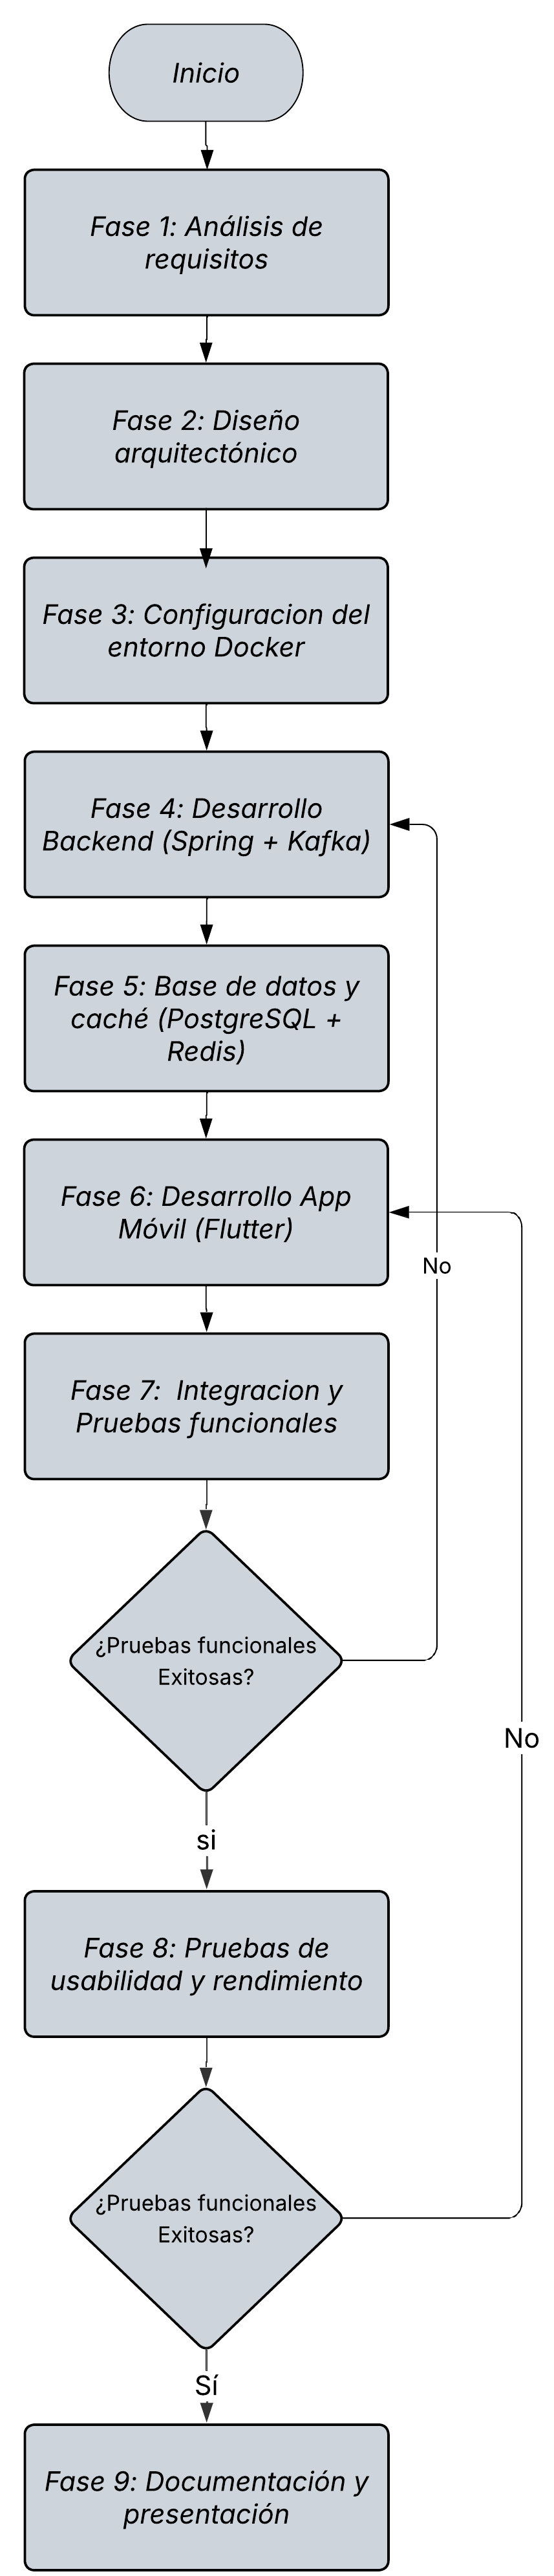
\includegraphics[width=0.20\textwidth]{imagenes/metodologia_flujo.png}
\caption{Flujo metodológico de las fases incrementales. Las flechas de retroalimentación indican ciclos de mejora.}
\label{fig:metodologia_flujo}
\end{figure}

\begin{figure}[H]
\centering
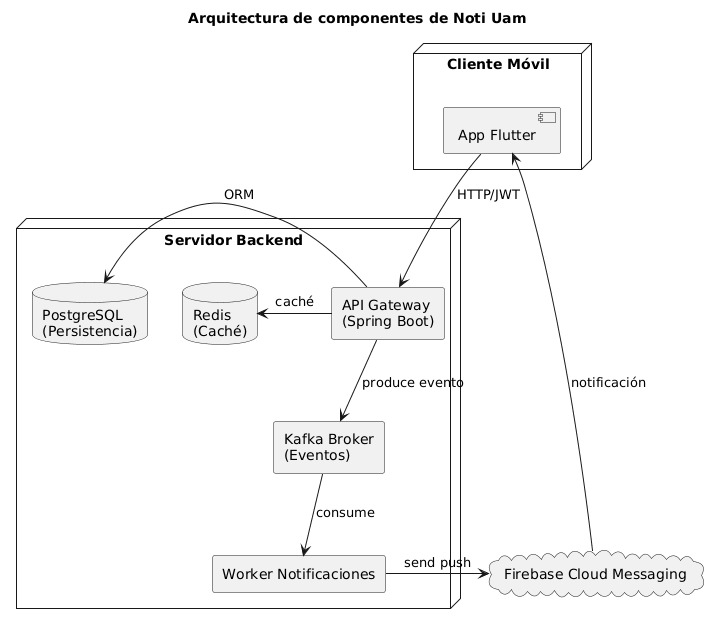
\includegraphics[width=0.30\textwidth]{imagenes/arquitectura_componentes.png}
\caption{Arquitectura de componentes de Noti Uam. El API Gateway recibe peticiones, publica eventos en Kafka; el Worker consume y envía notificaciones push.}
\label{fig:arquitectura}
\end{figure}

\begin{figure}[H]
\centering
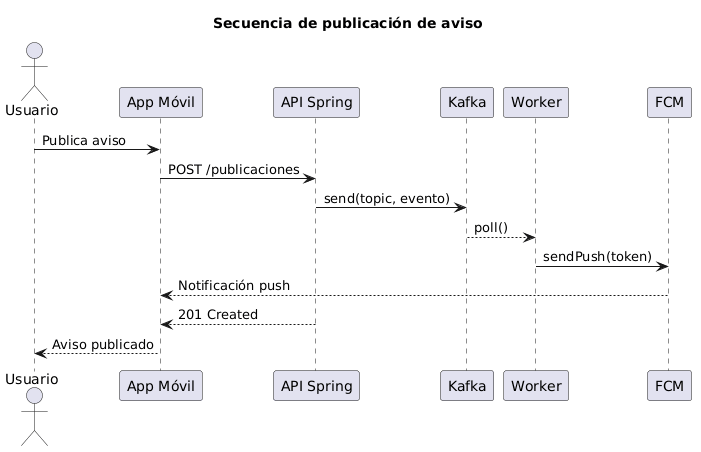
\includegraphics[width=0.30\textwidth]{imagenes/secuencia_publicacion.png}
\caption{Secuencia de publicación de un aviso y entrega de notificación push a suscriptores.}
\label{fig:secuencia}
\end{figure}

\begin{figure}[H]
\centering
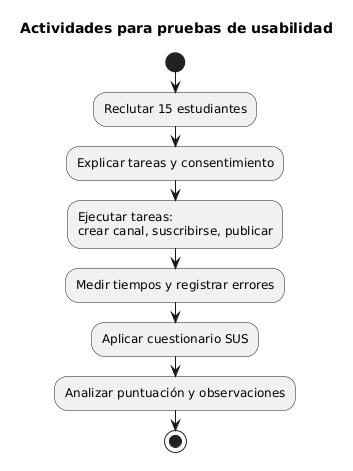
\includegraphics[width=0.35\textwidth]{imagenes/actividades_usabilidad.png}
\caption{Actividades para las pruebas de usabilidad con estudiantes.}
\label{fig:usabilidad}
\end{figure}

\subsection{Gestión de riesgos y contingencias}

La siguiente tabla identifica los principales riesgos técnicos y organizacionales, junto con sus planes de mitigación.

\begin{table}[H]
\centering
\caption{Riesgos y planes de mitigación}
\label{tab:riesgos}
\small
\begin{tabular}{|p{2cm}|p{2cm}|p{2cm}|}
\hline
\textbf{Riesgo} & \textbf{Impacto} & \textbf{Mitigación} \\
\hline
Fallo del broker Kafka & Pérdida de eventos en tiempo real & Configurar replicación de particiones y monitoreo con Prometheus; respaldo con Redis Streams como alternativa. \\
\hline
Alta latencia en notificaciones push & Mala experiencia de usuario & Optimizar la integración con FCM; usar colas de prioridad en Kafka. \\
\hline
Baja adopción en pruebas de usabilidad & Muestra insuficiente para validar hipótesis & Ofrecer incentivos; coordinar con profesores para solicitud de apoyo a la comunidad. \\
\hline
Problemas de compatibilidad entre Flutter y versiones de iOS/Android & Fallos en dispositivos reales & Probar en múltiples emuladores y dispositivos prestados; usar pruebas en la nube (Firebase Test Lab). \\
\hline
Sobrecarga de trabajo en el trimestre & Retraso en entregas & Priorizar funcionalidades críticas (MVP); aplicar metodología incremental para entregar al menos un prototipo funcional. \\
\hline
\end{tabular}
\end{table}

\subsection{Herramientas de desarrollo y colaboración}

\begin{itemize}
    \item \textbf{Control de versiones}: Git + GitHub (repositorio privado).
    \item \textbf{Gestión de tareas}: GitHub Projects o Trello, con etiquetas por fase.
    \item \textbf{CI/CD}: GitHub Actions para ejecutar pruebas unitarias automáticamente en cada \textit{push}.
    \item \textbf{Comunicación}: Discord / Slack para comunicación con el asesor.
    \item \textbf{Documentación}: Overleaf (LaTeX) para el informe y manuales.
    \item \textbf{Diagramas}: PlantUML (online) exportado a PNG.
\end{itemize}

\subsection{Criterios de aceptación final del proyecto}

Para dar por concluido el proyecto terminal, el sistema deberá cumplir con la siguiente lista de verificación:

\begin{enumerate}
    \item Todos los objetivos específicos se han alcanzado según lo documentado en las fases.
    \item La hipótesis general ha sido validada (o refutada, pero con conclusiones claras).
    \item El código fuente está disponible en un repositorio Git con un README que explique cómo ejecutar el sistema.
    \item El sistema se puede desplegar con \texttt{docker-compose up} en una máquina limpia.
    \item La puntuación SUS media es superior a 70.
    \item La documentación final (Protocolos I, II, III) ha sido aprobada por el asesor y otras autoridades pertinentes.
\end{enumerate}

La metodología descrita garantiza un desarrollo sistemático, trazable y orientado a la validación de la hipótesis, lo que es esencial para el éxito del proyecto terminal.